% Options for packages loaded elsewhere
% Options for packages loaded elsewhere
\PassOptionsToPackage{unicode}{hyperref}
\PassOptionsToPackage{hyphens}{url}
\PassOptionsToPackage{dvipsnames,svgnames,x11names}{xcolor}
%
\documentclass[
  letterpaper,
  DIV=11,
  numbers=noendperiod]{scrartcl}
\usepackage{xcolor}
\usepackage{amsmath,amssymb}
\setcounter{secnumdepth}{-\maxdimen} % remove section numbering
\usepackage{iftex}
\ifPDFTeX
  \usepackage[T1]{fontenc}
  \usepackage[utf8]{inputenc}
  \usepackage{textcomp} % provide euro and other symbols
\else % if luatex or xetex
  \usepackage{unicode-math} % this also loads fontspec
  \defaultfontfeatures{Scale=MatchLowercase}
  \defaultfontfeatures[\rmfamily]{Ligatures=TeX,Scale=1}
\fi
\usepackage{lmodern}
\ifPDFTeX\else
  % xetex/luatex font selection
\fi
% Use upquote if available, for straight quotes in verbatim environments
\IfFileExists{upquote.sty}{\usepackage{upquote}}{}
\IfFileExists{microtype.sty}{% use microtype if available
  \usepackage[]{microtype}
  \UseMicrotypeSet[protrusion]{basicmath} % disable protrusion for tt fonts
}{}
\makeatletter
\@ifundefined{KOMAClassName}{% if non-KOMA class
  \IfFileExists{parskip.sty}{%
    \usepackage{parskip}
  }{% else
    \setlength{\parindent}{0pt}
    \setlength{\parskip}{6pt plus 2pt minus 1pt}}
}{% if KOMA class
  \KOMAoptions{parskip=half}}
\makeatother
% Make \paragraph and \subparagraph free-standing
\makeatletter
\ifx\paragraph\undefined\else
  \let\oldparagraph\paragraph
  \renewcommand{\paragraph}{
    \@ifstar
      \xxxParagraphStar
      \xxxParagraphNoStar
  }
  \newcommand{\xxxParagraphStar}[1]{\oldparagraph*{#1}\mbox{}}
  \newcommand{\xxxParagraphNoStar}[1]{\oldparagraph{#1}\mbox{}}
\fi
\ifx\subparagraph\undefined\else
  \let\oldsubparagraph\subparagraph
  \renewcommand{\subparagraph}{
    \@ifstar
      \xxxSubParagraphStar
      \xxxSubParagraphNoStar
  }
  \newcommand{\xxxSubParagraphStar}[1]{\oldsubparagraph*{#1}\mbox{}}
  \newcommand{\xxxSubParagraphNoStar}[1]{\oldsubparagraph{#1}\mbox{}}
\fi
\makeatother

\usepackage{color}
\usepackage{fancyvrb}
\newcommand{\VerbBar}{|}
\newcommand{\VERB}{\Verb[commandchars=\\\{\}]}
\DefineVerbatimEnvironment{Highlighting}{Verbatim}{commandchars=\\\{\}}
% Add ',fontsize=\small' for more characters per line
\usepackage{framed}
\definecolor{shadecolor}{RGB}{241,243,245}
\newenvironment{Shaded}{\begin{snugshade}}{\end{snugshade}}
\newcommand{\AlertTok}[1]{\textcolor[rgb]{0.68,0.00,0.00}{#1}}
\newcommand{\AnnotationTok}[1]{\textcolor[rgb]{0.37,0.37,0.37}{#1}}
\newcommand{\AttributeTok}[1]{\textcolor[rgb]{0.40,0.45,0.13}{#1}}
\newcommand{\BaseNTok}[1]{\textcolor[rgb]{0.68,0.00,0.00}{#1}}
\newcommand{\BuiltInTok}[1]{\textcolor[rgb]{0.00,0.23,0.31}{#1}}
\newcommand{\CharTok}[1]{\textcolor[rgb]{0.13,0.47,0.30}{#1}}
\newcommand{\CommentTok}[1]{\textcolor[rgb]{0.37,0.37,0.37}{#1}}
\newcommand{\CommentVarTok}[1]{\textcolor[rgb]{0.37,0.37,0.37}{\textit{#1}}}
\newcommand{\ConstantTok}[1]{\textcolor[rgb]{0.56,0.35,0.01}{#1}}
\newcommand{\ControlFlowTok}[1]{\textcolor[rgb]{0.00,0.23,0.31}{\textbf{#1}}}
\newcommand{\DataTypeTok}[1]{\textcolor[rgb]{0.68,0.00,0.00}{#1}}
\newcommand{\DecValTok}[1]{\textcolor[rgb]{0.68,0.00,0.00}{#1}}
\newcommand{\DocumentationTok}[1]{\textcolor[rgb]{0.37,0.37,0.37}{\textit{#1}}}
\newcommand{\ErrorTok}[1]{\textcolor[rgb]{0.68,0.00,0.00}{#1}}
\newcommand{\ExtensionTok}[1]{\textcolor[rgb]{0.00,0.23,0.31}{#1}}
\newcommand{\FloatTok}[1]{\textcolor[rgb]{0.68,0.00,0.00}{#1}}
\newcommand{\FunctionTok}[1]{\textcolor[rgb]{0.28,0.35,0.67}{#1}}
\newcommand{\ImportTok}[1]{\textcolor[rgb]{0.00,0.46,0.62}{#1}}
\newcommand{\InformationTok}[1]{\textcolor[rgb]{0.37,0.37,0.37}{#1}}
\newcommand{\KeywordTok}[1]{\textcolor[rgb]{0.00,0.23,0.31}{\textbf{#1}}}
\newcommand{\NormalTok}[1]{\textcolor[rgb]{0.00,0.23,0.31}{#1}}
\newcommand{\OperatorTok}[1]{\textcolor[rgb]{0.37,0.37,0.37}{#1}}
\newcommand{\OtherTok}[1]{\textcolor[rgb]{0.00,0.23,0.31}{#1}}
\newcommand{\PreprocessorTok}[1]{\textcolor[rgb]{0.68,0.00,0.00}{#1}}
\newcommand{\RegionMarkerTok}[1]{\textcolor[rgb]{0.00,0.23,0.31}{#1}}
\newcommand{\SpecialCharTok}[1]{\textcolor[rgb]{0.37,0.37,0.37}{#1}}
\newcommand{\SpecialStringTok}[1]{\textcolor[rgb]{0.13,0.47,0.30}{#1}}
\newcommand{\StringTok}[1]{\textcolor[rgb]{0.13,0.47,0.30}{#1}}
\newcommand{\VariableTok}[1]{\textcolor[rgb]{0.07,0.07,0.07}{#1}}
\newcommand{\VerbatimStringTok}[1]{\textcolor[rgb]{0.13,0.47,0.30}{#1}}
\newcommand{\WarningTok}[1]{\textcolor[rgb]{0.37,0.37,0.37}{\textit{#1}}}

\usepackage{longtable,booktabs,array}
\newcounter{none} % for unnumbered tables
\usepackage{calc} % for calculating minipage widths
% Correct order of tables after \paragraph or \subparagraph
\usepackage{etoolbox}
\makeatletter
\patchcmd\longtable{\par}{\if@noskipsec\mbox{}\fi\par}{}{}
\makeatother
% Allow footnotes in longtable head/foot
\IfFileExists{footnotehyper.sty}{\usepackage{footnotehyper}}{\usepackage{footnote}}
\makesavenoteenv{longtable}
\usepackage{graphicx}
\makeatletter
\newsavebox\pandoc@box
\newcommand*\pandocbounded[1]{% scales image to fit in text height/width
  \sbox\pandoc@box{#1}%
  \Gscale@div\@tempa{\textheight}{\dimexpr\ht\pandoc@box+\dp\pandoc@box\relax}%
  \Gscale@div\@tempb{\linewidth}{\wd\pandoc@box}%
  \ifdim\@tempb\p@<\@tempa\p@\let\@tempa\@tempb\fi% select the smaller of both
  \ifdim\@tempa\p@<\p@\scalebox{\@tempa}{\usebox\pandoc@box}%
  \else\usebox{\pandoc@box}%
  \fi%
}
% Set default figure placement to htbp
\def\fps@figure{htbp}
\makeatother





\setlength{\emergencystretch}{3em} % prevent overfull lines

\providecommand{\tightlist}{%
  \setlength{\itemsep}{0pt}\setlength{\parskip}{0pt}}



 


\KOMAoption{captions}{tableheading}
\usepackage{tcolorbox}
\tcbuselibrary{skins,breakable}
\definecolor{embernavy}{HTML}{0D1B2A}
\definecolor{emberamber}{HTML}{C8762A}
\definecolor{emberrule}{HTML}{E0D8CC}
\definecolor{emberborder}{HTML}{D8CEBC}
\newtcolorbox{slidebox}{%
  enhanced, breakable, colback=white, colframe=emberborder,
  boxrule=0.4pt, arc=1.5pt,
  left=10pt, right=10pt, top=9pt, bottom=9pt,
  borderline north={2.5pt}{0pt}{emberamber},
}
\newcommand{\slidelabel}[1]{{\color{embernavy}\bfseries\large #1\par\vspace{5pt}}}
\newenvironment{slidefooter}{%
  \par\vspace{7pt}{\color{emberrule}\rule{\linewidth}{0.4pt}}\par\vspace{4pt}%
  \color{emberamber}\itshape\small}{\par}
\makeatletter
\@ifpackageloaded{tcolorbox}{}{\usepackage[skins,breakable]{tcolorbox}}
\@ifpackageloaded{fontawesome5}{}{\usepackage{fontawesome5}}
\definecolor{quarto-callout-color}{HTML}{909090}
\definecolor{quarto-callout-note-color}{HTML}{0758E5}
\definecolor{quarto-callout-important-color}{HTML}{CC1914}
\definecolor{quarto-callout-warning-color}{HTML}{EB9113}
\definecolor{quarto-callout-tip-color}{HTML}{00A047}
\definecolor{quarto-callout-caution-color}{HTML}{FC5300}
\definecolor{quarto-callout-color-frame}{HTML}{acacac}
\definecolor{quarto-callout-note-color-frame}{HTML}{4582ec}
\definecolor{quarto-callout-important-color-frame}{HTML}{d9534f}
\definecolor{quarto-callout-warning-color-frame}{HTML}{f0ad4e}
\definecolor{quarto-callout-tip-color-frame}{HTML}{02b875}
\definecolor{quarto-callout-caution-color-frame}{HTML}{fd7e14}
\makeatother
\makeatletter
\@ifpackageloaded{caption}{}{\usepackage{caption}}
\AtBeginDocument{%
\ifdefined\contentsname
  \renewcommand*\contentsname{Table of contents}
\else
  \newcommand\contentsname{Table of contents}
\fi
\ifdefined\listfigurename
  \renewcommand*\listfigurename{List of Figures}
\else
  \newcommand\listfigurename{List of Figures}
\fi
\ifdefined\listtablename
  \renewcommand*\listtablename{List of Tables}
\else
  \newcommand\listtablename{List of Tables}
\fi
\ifdefined\figurename
  \renewcommand*\figurename{Figure}
\else
  \newcommand\figurename{Figure}
\fi
\ifdefined\tablename
  \renewcommand*\tablename{Table}
\else
  \newcommand\tablename{Table}
\fi
}
\@ifpackageloaded{float}{}{\usepackage{float}}
\floatstyle{ruled}
\@ifundefined{c@chapter}{\newfloat{codelisting}{h}{lop}}{\newfloat{codelisting}{h}{lop}[chapter]}
\floatname{codelisting}{Listing}
\newcommand*\listoflistings{\listof{codelisting}{List of Listings}}
\makeatother
\makeatletter
\makeatother
\makeatletter
\@ifpackageloaded{caption}{}{\usepackage{caption}}
\@ifpackageloaded{subcaption}{}{\usepackage{subcaption}}
\makeatother
\usepackage{bookmark}
\IfFileExists{xurl.sty}{\usepackage{xurl}}{} % add URL line breaks if available
\urlstyle{same}
\hypersetup{
  pdftitle={Introducing ARMA(p{,} q) models},
  colorlinks=true,
  linkcolor={blue},
  filecolor={Maroon},
  citecolor={Blue},
  urlcolor={Blue},
  pdfcreator={LaTeX via pandoc}}


\title{Introducing ARMA(p, q) models}
\usepackage{etoolbox}
\makeatletter
\providecommand{\subtitle}[1]{% add subtitle to \maketitle
  \apptocmd{\@title}{\par {\large #1 \par}}{}{}
}
\makeatother
\subtitle{Topic 2}
\author{}
\date{}
\begin{document}
\maketitle


{Goals}

\begin{itemize}
\tightlist
\item
  To look at some simple time series plots
\item
  To introduce \(\mathsf{WN}\), \(\mathsf{MA}\) and \(\mathsf{AR}\)
  models
\item
  To define \(\mathsf{ARMA}(p, q)\) models
\item
  To understand the lag operator and polynomials in the lag operator
\end{itemize}

{Key Equation}

\[\Phi(L) Y_t = \Theta(L)\varepsilon_t, \text{ where } \varepsilon_t \sim \mathsf{WN}(0, \sigma_\varepsilon^2) \text{ and } \Phi(L) \text{ and } \Theta(L) \text{ are lag polynomials}\]

\begin{center}\rule{0.5\linewidth}{0.5pt}\end{center}

\subsection{Examples of time series
plots}\label{examples-of-time-series-plots}

\begin{itemize}
\tightlist
\item
  We learned that one primary objective of time series analysis is to
  develop statistical models that provide plausible descriptions for
  data that are temporally ordered. Let us look at an
  (arbitrarily-chosen) example now.
\end{itemize}

\begin{figure}[H]

{\centering \pandocbounded{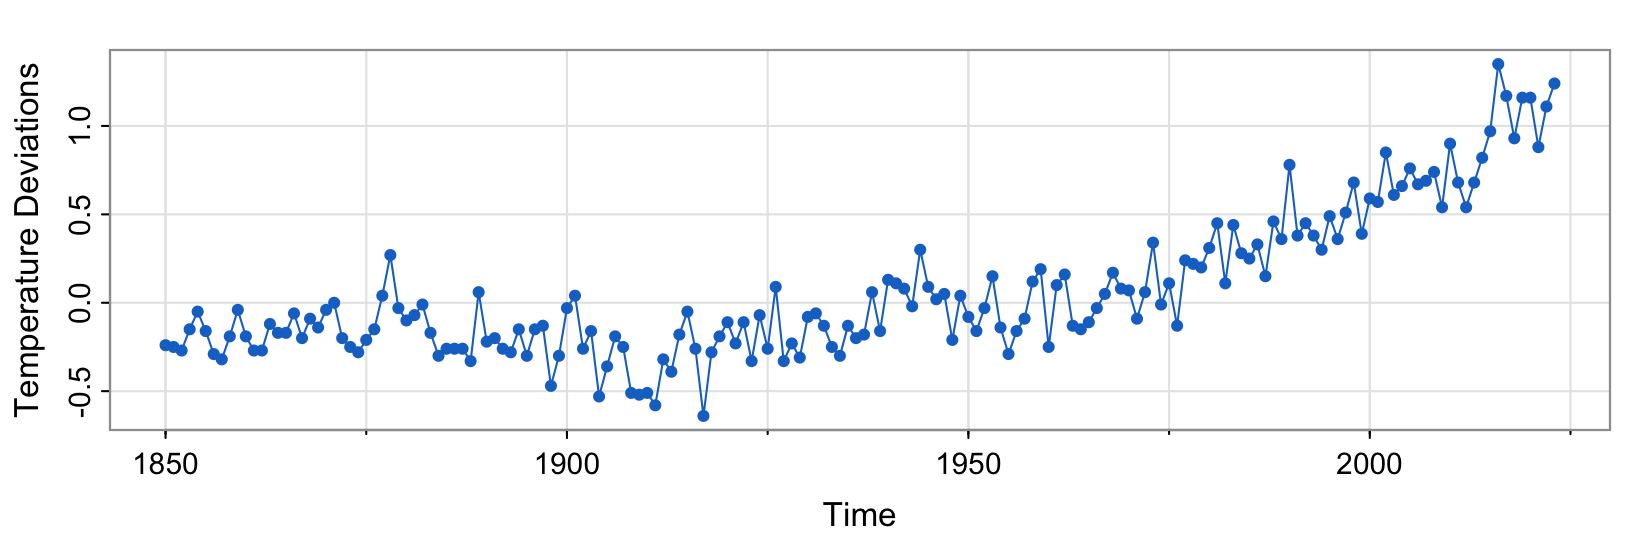
\includegraphics[keepaspectratio]{sample_globaltemp.png}}

}

\caption{Yearly average global temperature deviations (1880--2015) in
degrees centigrade.}

\end{figure}%

\begin{itemize}
\item
  Notice that it is conventional, when displaying such data graphically,
  to plot the values of the data points on the vertical or \(y\) axis,
  with the time scale on the horizontal or \(x\) axis. It is also common
  practice to connect the values at adjacent time periods to reconstruct
  visually some original hypothetical continuous time series that might
  have produced these values as a discrete sample.\footnote{Although we
    plot data in this fashion, note that (i) we will NOT study
    continuous time series models in this course (nevertheless, do be
    aware that they comprise an entire field of study in financial
    modelling --- e.g.~for use in option pricing and/or high-frequency
    trading); and (ii) we will NOT get into issues surrounding selection
    of the sampling rate when discretising a continuous time series even
    though these issues can be extremely important.}
\item
  To formally characterise data that seemingly fluctuate in random
  fashion over time, statisticians assume that any real-life sample
  considered is obtained as a realisation of a collection of random
  variables (i.e.~a stochastic process) indexed according to the order
  they are obtained in time.
\item
  For example, we may consider as a time series the sequence of random
  variables, \(Y_1, Y_2, Y_3, \ldots\), where \(Y_1\) denotes the value
  taken by the series at the first time point, the variable \(Y_2\)
  denotes the value for the second time point, and so on. The stochastic
  process is denoted \(\{Y_t\}\). Note that in all our lectures, \(t\)
  will be discrete and vary over the integers,
  \(t = 0, \pm 1, \pm 2, \ldots\), or some subset of the integers, such
  as \(t = 1, \ldots, T\). It will also be assumed that our observations
  are spaced equally.
\item
  The next step is to \textbf{understand how to specify a (parametric)
  statistical model that suitably characterises the inter-temporal
  dependence structure} between the random variables within the
  (presumably stable) stochastic process. These are the models we will
  study shortly. (We will subsequently also explore the key ideas behind
  model selection and parameter estimation.)
\item
  On the next page, we briefly contemplate the visual patterns that
  arise in a few more examples of time series data (chosen by me for
  reasons that will become clearer in future weeks). In case you are
  interested, the contextual details about these graphs are in
  \textbf{SS (Chapter 1.1)}.
\end{itemize}

\begin{figure}[H]

{\centering \pandocbounded{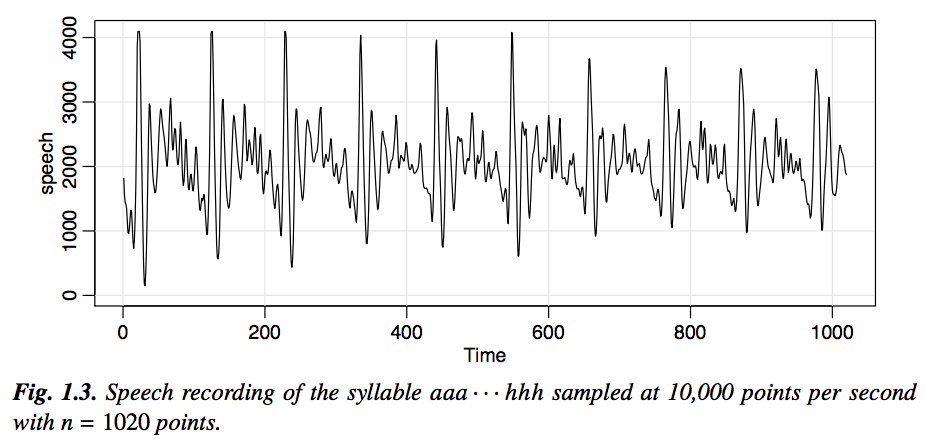
\includegraphics[keepaspectratio]{sample_speech.png}}

}

\caption{Speech recording of the syllable aaa···hhh sampled at 10,000
points per second with n = 1020 points.}

\end{figure}%

\begin{figure}[H]

{\centering \pandocbounded{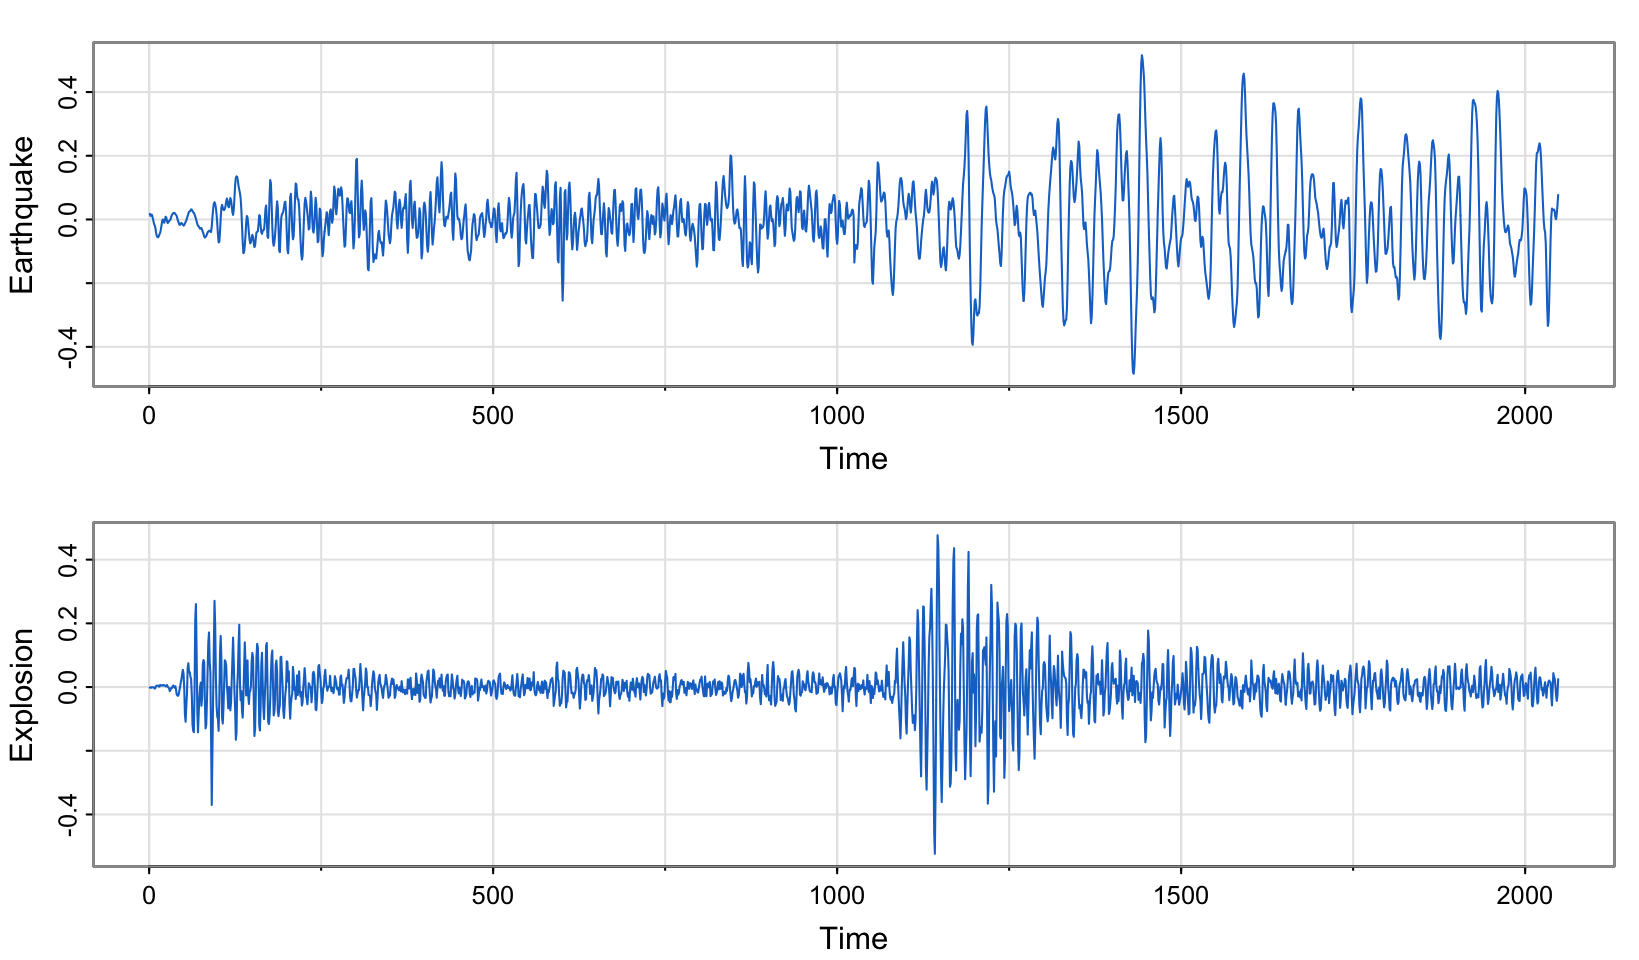
\includegraphics[keepaspectratio]{sample_disaster.png}}

}

\caption{Arrival phases from an earthquake (top) and explosion (bottom)
at 40 points per second.}

\end{figure}%

\begin{figure}[H]

{\centering \pandocbounded{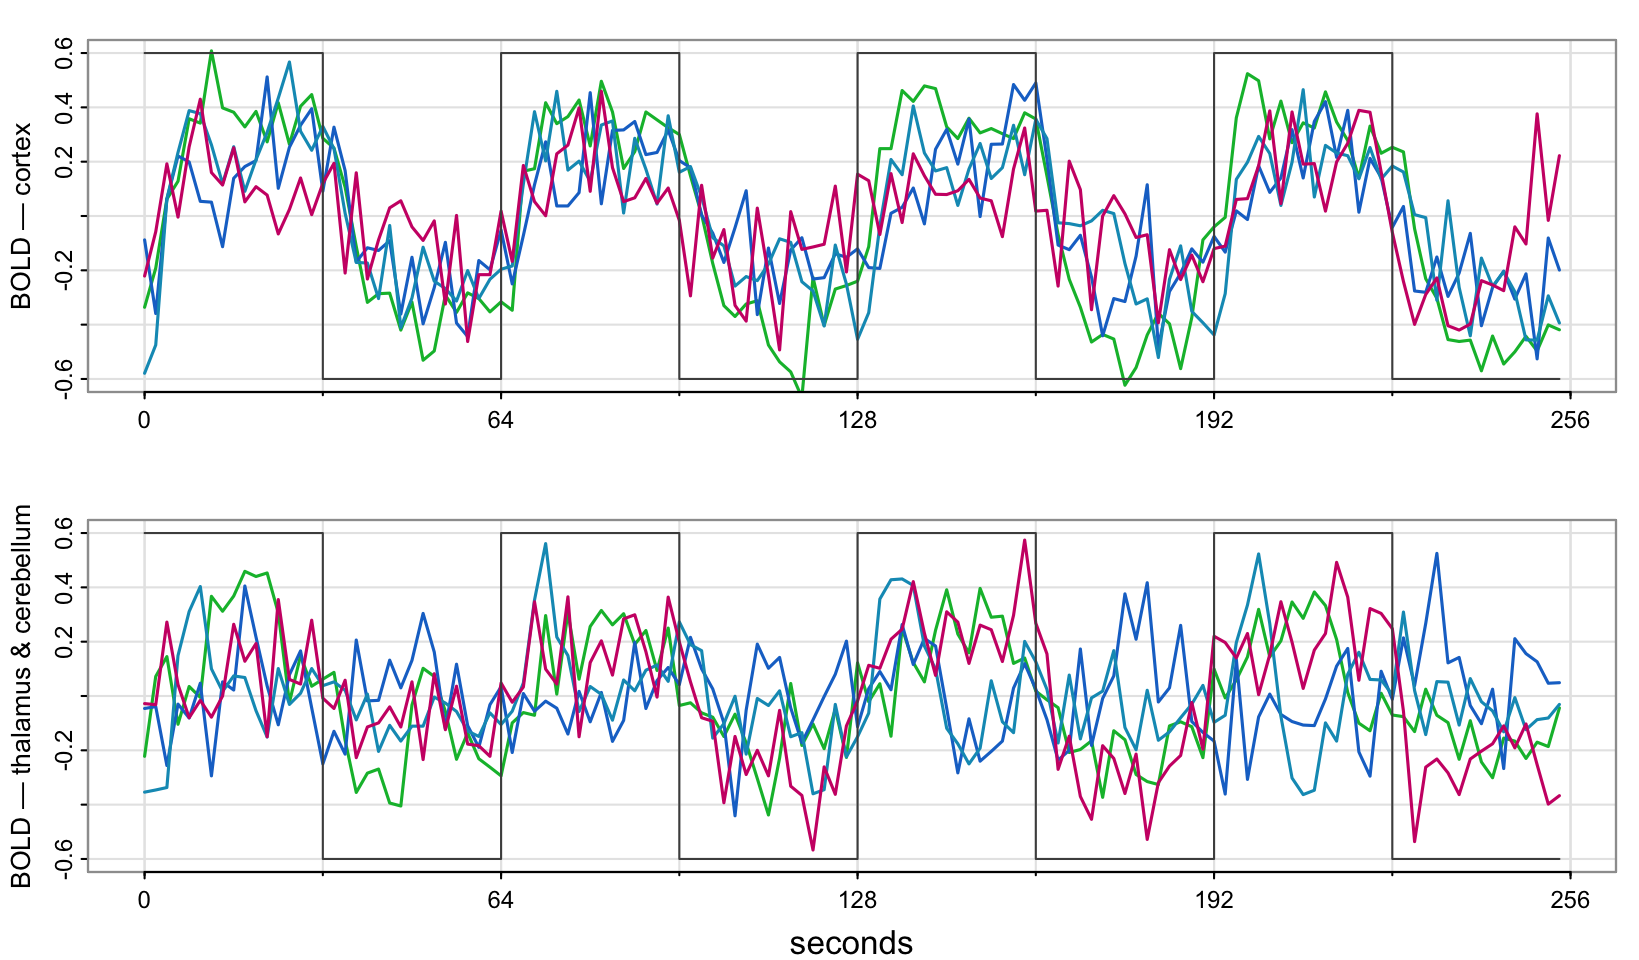
\includegraphics[keepaspectratio]{sample_fmri.png}}

}

\caption{fMRI data from various locations in the cortex, thalamus, and
cerebellum; n = 128 points, one observation taken every 2 seconds.}

\end{figure}%

\pandocbounded{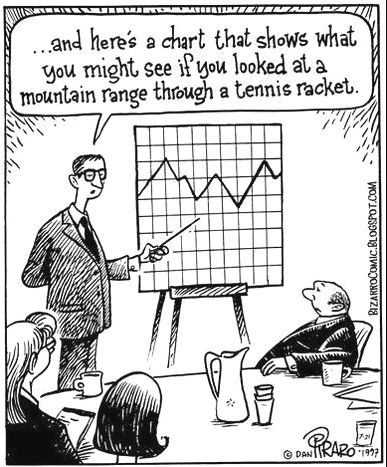
\includegraphics[keepaspectratio]{mountain.jpeg}}

\begin{center}\rule{0.5\linewidth}{0.5pt}\end{center}

\subsection{Building blocks of the ARMA
framework}\label{building-blocks-of-the-arma-framework}

\begin{slidebox}

\slidelabel{What is a white noise process?}

\textbf{Definition.} Consider a stochastic process \(\{Y_t\}\) where
\(\mathsf{E}(Y_t) = \mu_Y\) and
\[\text{Cov}(Y_t, Y_s) = \begin{cases} 0 < \sigma_Y^2 < \infty, & t = s, \\ 0, & \text{otherwise} \end{cases}\]
for \(t, s \in \mathbb{Z}\). We say that \(\{Y_t\}\) is a white noise
process with mean \(\mu_Y\) and variance \(\sigma_Y^2\), or simply
\(Y_t \sim \mathsf{WN}\left(\mu_Y, \sigma_Y^2\right)\). (The mean
\(\mu_Y\) is most often assumed zero.) \(\qquad\square\)

\begin{itemize}
\tightlist
\item
  A white noise process (or informally, just ``noise'') is a collection
  of time-ordered yet \textbf{uncorrelated} random variables. An example
  would be the typical
  \(Y_t \overset{\scriptscriptstyle\text{iid}}{\sim} \mathcal{N}\left(\mu_Y, \sigma_Y^2\right),\ t \in \mathbb{Z}\)
  process that you've worked with but note that neither is normality (or
  ``Gaussianity'') nor is the \(iid\) assumption needed for a process to
  be classified as noise.
\end{itemize}

\begin{slidefooter}

A collection of time-ordered yet uncorrelated random variables.

\end{slidefooter}

\end{slidebox}

\begin{slidebox}

\slidelabel{How is noise even relevant? Are we not studying dependent
processes?}

\begin{itemize}
\item
  The perceptive student may wonder why a white noise process gets prime
  billing in a course whose central concern is serial correlation. It
  seems odd, does it not? Indeed, if the stochastic behaviour of all
  time series could be explained in terms of the white noise model,
  classical statistical methods would suffice!
\item
  I would like you to appreciate that one of the key features of the
  \(\mathsf{ARMA}\) framework (which we are about to study) is that even
  \textbf{processes with highly-sophisticated dependence structures can
  be built just by linearly combining --- or in time series parlance,
  ``filtering'' through --- uncorrelated random variables}. The simple
  white noise process thus serves as the springboard for the rest of the
  theory, and this is truly remarkable!
\item
  Let's see how it works. Ways of introducing dynamics are discussed
  below. But first, let us define a linear filter\ldots{}
\end{itemize}

\begin{slidefooter}

Noise is the springboard: rich dependence is built by filtering
uncorrelated random variables.

\end{slidefooter}

\end{slidebox}

Terms and phrases commonly-used in place of ``dynamics'' that you might
encounter in your studies include ``inter-temporal dependence'',
``persistence'', ``smoothness'', and ``inertia'', to name a few.

\begin{slidebox}

\slidelabel{What is a linear filter?}

A linear (time-invariant) filter or ``smoother'' converts one time
series, \(\{\varepsilon_t\}\), into another, \(\{Y_t\}\), by the linear
operation \[Y_t = \sum_{h=-q}^{+s} a_h\,\varepsilon_{t+h},\] where
\(\{a_h\}\), for \(h = -q, \ldots, s\) is a set of weights for
\(q, s \in \mathbb{N}\). Notice that the filter is symmetric when
\(s = q\) and \(a_h = a_{-h}\).

\begin{itemize}
\item
  Formally, a linear filter is a polynomial in the lag operator, but we
  will see the formal definition after we introduce the concept of a lag
  operator (in \hyperref[the-arma-framework]{The ARMA framework} below).
\item
  The simplest example of a two-sided symmetric filter is when
  \[a_h = \begin{cases} \frac{1}{2q+1}, & h \in \{-q, \ldots, 0, \ldots, q\} \\ 0, & \text{otherwise}, \end{cases}\]
  so that the filtered value of \(Y_t\) is given by
  \[Y_t = \frac{1}{2q+1}\sum_{h=-q}^{q}\varepsilon_{t+h}.\]
\item
  Can you try to visualise the given operation and determine for
  yourself why a linear filter might synonymously be referred to as a
  smoother?
\end{itemize}

\begin{slidefooter}

A weighted sum of neighbouring noise terms; equal weights give a
smoother.

\end{slidefooter}

\end{slidebox}

Consider, for example,
\(Y_t = (\varepsilon_{t-1} + \varepsilon_t + \varepsilon_{t+1})/3\). We
have the following schematic to help describe this two-sided symmetric
smoothing operation:

\[\begin{aligned} \underset{Y_2}{\underbrace{\tfrac{1}{3}\varepsilon_1 \quad \tfrac{1}{3}\varepsilon_2 \quad \tfrac{1}{3}\varepsilon_3}} \quad \varepsilon_4 \quad \varepsilon_5 \\ \varepsilon_1 \quad \underset{Y_3}{\underbrace{\tfrac{1}{3}\varepsilon_2 \quad \tfrac{1}{3}\varepsilon_3 \quad \tfrac{1}{3}\varepsilon_4}} \quad \varepsilon_5 \\ \varepsilon_1 \quad \varepsilon_2 \quad \underset{Y_4}{\underbrace{\tfrac{1}{3}\varepsilon_3 \quad \tfrac{1}{3}\varepsilon_4 \quad \tfrac{1}{3}\varepsilon_5}} \end{aligned}\]

Do you see how we created a completely new series,
\(\{Y_2, Y_3, Y_4\}\), from the original,
\(\{\varepsilon_1, \varepsilon_2, \varepsilon_3, \varepsilon_4, \varepsilon_5\}\)?

Let us look at some graphs that help illustrate the distinction between
white noise and the three-point moving average process above.

\begin{figure}[H]

{\centering \pandocbounded{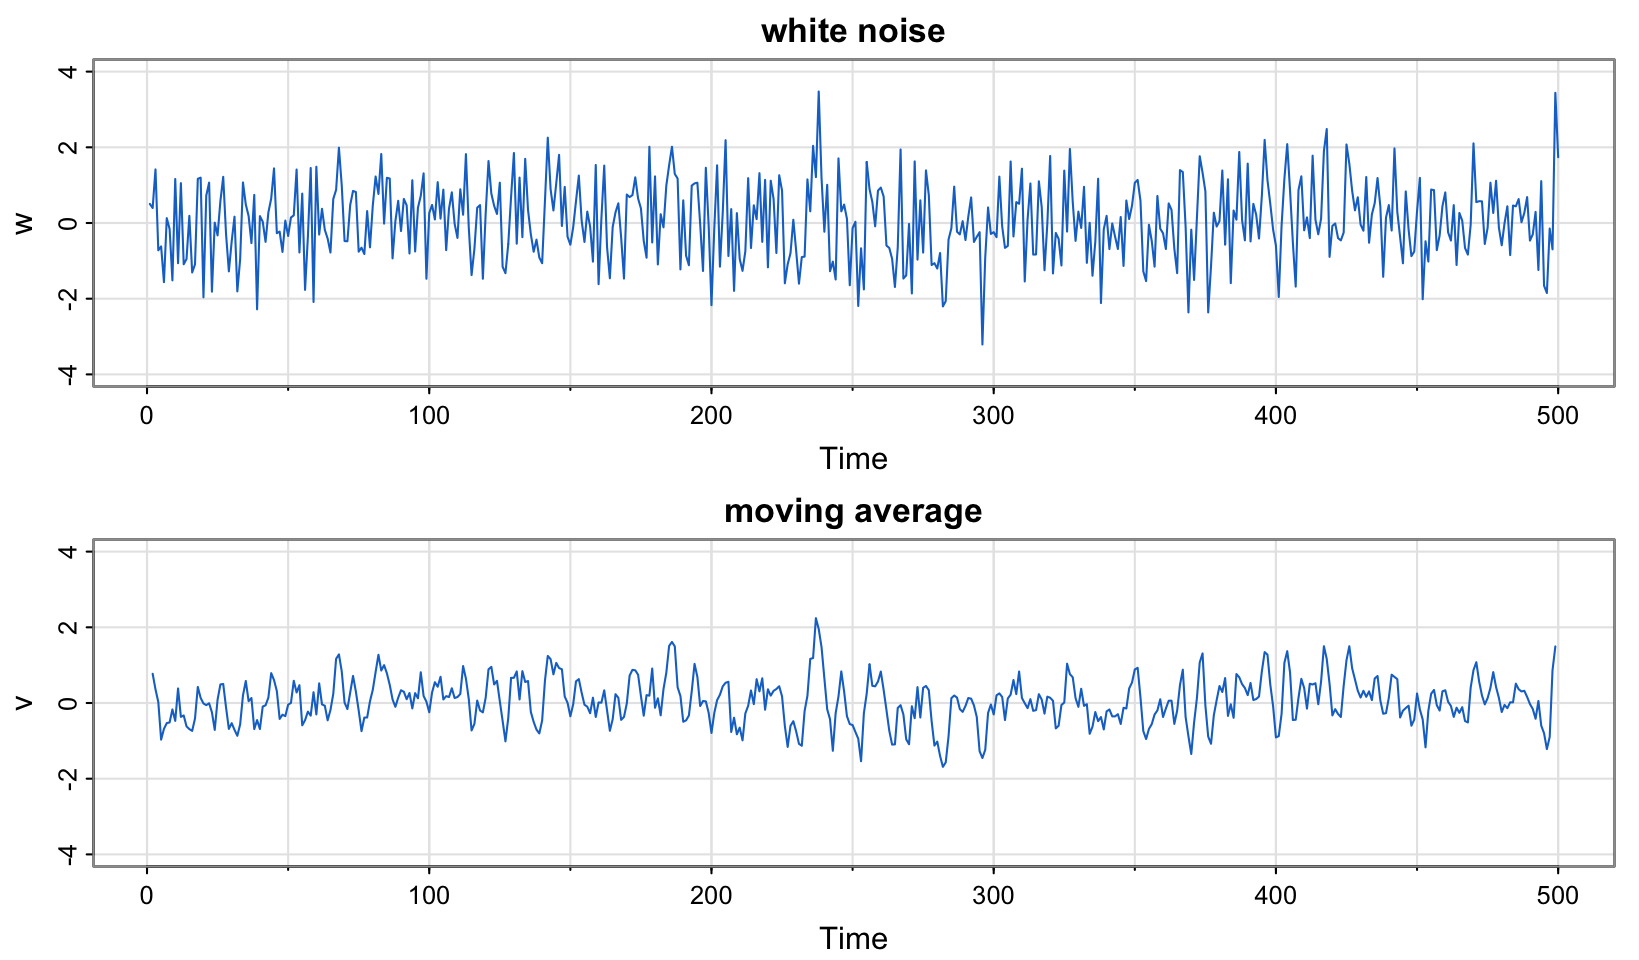
\includegraphics[keepaspectratio]{sample_wnma.png}}

}

\caption{Gaussian white noise series (top) and three-point moving
average of the Gaussian white noise series (bottom).}

\end{figure}%

\begin{Shaded}
\begin{Highlighting}[]
\SpecialCharTok{\textgreater{}}\NormalTok{ w }\OtherTok{=} \FunctionTok{rnorm}\NormalTok{(}\DecValTok{500}\NormalTok{,}\DecValTok{0}\NormalTok{,}\DecValTok{1}\NormalTok{) }\CommentTok{\# creates realisations of 500 iid N(0,1) RVs}
\SpecialCharTok{\textgreater{}}\NormalTok{ v }\OtherTok{=} \FunctionTok{filter}\NormalTok{(w, }\AttributeTok{sides=}\DecValTok{2}\NormalTok{, }\AttributeTok{filter=}\FunctionTok{rep}\NormalTok{(}\DecValTok{1}\SpecialCharTok{/}\DecValTok{3}\NormalTok{,}\DecValTok{3}\NormalTok{)) }\CommentTok{\# creates a moving average}
\SpecialCharTok{\textgreater{}} \FunctionTok{par}\NormalTok{(}\AttributeTok{mfrow=}\FunctionTok{c}\NormalTok{(}\DecValTok{2}\NormalTok{,}\DecValTok{1}\NormalTok{)) }\CommentTok{\# specifies a 2 by 1 panel layout for graphs}
\SpecialCharTok{\textgreater{}} \FunctionTok{plot.ts}\NormalTok{(w, }\AttributeTok{main=}\StringTok{"white noise"}\NormalTok{)}
\SpecialCharTok{\textgreater{}} \FunctionTok{plot.ts}\NormalTok{(v, }\AttributeTok{ylim=}\FunctionTok{c}\NormalTok{(}\SpecialCharTok{{-}}\DecValTok{3}\NormalTok{,}\DecValTok{3}\NormalTok{), }\AttributeTok{main=}\StringTok{"moving average"}\NormalTok{)}
\end{Highlighting}
\end{Shaded}

Consider, as a different example of a moving average,
\(Y_t = \varepsilon_t + 0.5\varepsilon_{t-1}\). We have the following
schematic to help describe this one-sided smoothing operation:

\[\begin{aligned} \underset{Y_2}{\underbrace{0.5\,\varepsilon_1 \quad \varepsilon_2}} \quad \varepsilon_3 \quad \varepsilon_4 \quad \varepsilon_5 \\ \varepsilon_1 \quad \underset{Y_3}{\underbrace{0.5\,\varepsilon_2 \quad \varepsilon_3}} \quad \varepsilon_4 \quad \varepsilon_5 \\ \varepsilon_1 \quad \varepsilon_2 \quad \underset{Y_4}{\underbrace{0.5\,\varepsilon_3 \quad \varepsilon_4}} \quad \varepsilon_5 \\ \varepsilon_1 \quad \varepsilon_2 \quad \varepsilon_3 \quad \underset{Y_5}{\underbrace{0.5\,\varepsilon_4 \quad \varepsilon_5}} \end{aligned}\]

This example brings us now to the definition of \(\mathsf{MA}(q)\)
processes.

\begin{slidebox}

\slidelabel{What is an MA(q) process?}

\textbf{Definition.} A process \(\{Y_t\}\) is called a moving average
process of order \(q\), with shorthand \(Y_t \sim \mathsf{MA}(q)\), if
there exists a white noise process
\(\varepsilon_t \sim \mathsf{WN}\left(0, \sigma_\varepsilon^2\right)\)
and a set of finite constants \(\theta_j\), for \(j = 1, \ldots, q\),
with \(\theta_q \neq 0\), such that
\[Y_t = \varepsilon_t + \theta_1\varepsilon_{t-1} + \cdots + \theta_q\varepsilon_{t-q},\]
for \(t \in \mathbb{Z}\). \(\qquad\square\)

\begin{itemize}
\item
  An example (which we already saw) is the simple
  \textbf{\(\mathsf{MA}(1)\) process} given by
  \[Y_t = \varepsilon_t + 0.5\varepsilon_{t-1}\] where it is clear that
  \(Y_t\) is serially correlated, since
  \[\text{Cov}(Y_t, Y_{t-1}) = \text{Cov}(\varepsilon_t + 0.5\varepsilon_{t-1}, \varepsilon_{t-1} + 0.5\varepsilon_{t-2}) = 0.5\sigma_\varepsilon^2,\]
  even though
  \(\varepsilon_t \sim \mathsf{WN}\left(0, \sigma_\varepsilon^2\right)\).
\item
  It is worth re-emphasising that we have created in \(\{Y_t\}\) a
  completely new process that exhibits very different dependence
  characteristics from serially uncorrelated process
  \(\{\varepsilon_t\}\) just by linearly combining elements of the
  latter.
\end{itemize}

\begin{slidefooter}

A finite linear combination of current and past noise terms.

\end{slidefooter}

\end{slidebox}

Another way of introducing dynamics is by explicitly postulating a
linear relationship between a random variable, \(Y_t\), and its past
values, \(Y_{t-h}\) for \(h > 0\). These relationships are referred to
as autoregressions.

\begin{slidebox}

\slidelabel{What is an AR(p) process?}

\textbf{Definition.} A process \(\{Y_t\}\) is called an autoregressive
process of order \(p\), with shorthand \(Y_t \sim \mathsf{AR}(p)\), if
there exists a white noise process
\(\varepsilon_t \sim \mathsf{WN}\left(0, \sigma_\varepsilon^2\right)\)
and a set of finite constants \(\phi_j\), for \(j = 1, \ldots, p\), with
\(\phi_p \neq 0\), such that
\[Y_t = \phi_1 Y_{t-1} + \cdots + \phi_p Y_{t-p} + \varepsilon_t,\] for
\(t \in \mathbb{Z}\). \(\qquad\square\)

\begin{itemize}
\tightlist
\item
  An example is the \textbf{\(\mathsf{AR}(1)\) process} given by
  \[Y_t = \phi Y_{t-1} + \varepsilon_t, \qquad 0 < \phi < 1,\] where the
  introduction of dynamics (relative to the \(\mathsf{WN}\) case) can be
  illustrated by checking the autocovariances, which we will do in
  detail soon.
\end{itemize}

\begin{slidefooter}

The present regressed on its own finite past, plus noise.

\end{slidefooter}

\end{slidebox}

\begin{slidebox}

\slidelabel{Are we really just linearly combining noise again\ldots?}

Understand that yet again we are \textbf{filtering through noise} in
order to generate a complicated dynamic structure. To see this, try the
following exercise:

\[\begin{aligned} Y_t &= \phi Y_{t-1} + \varepsilon_t \\ &= \phi^2 Y_{t-2} + \phi\varepsilon_{t-1} + \varepsilon_t \quad \text{by lagging/substituting once,} \\ &= \phi^3 Y_{t-3} + \phi^2\varepsilon_{t-2} + \phi\varepsilon_{t-1} + \varepsilon_t \quad \text{by lagging/substituting twice,} \\ &= \ldots \\ &= \phi^{h+1} Y_{t-h-1} + \sum_{k=0}^{h}\phi^k\varepsilon_{t-k} \quad \text{by lagging/substituting } h > 2 \text{ times.} \end{aligned}\]

Letting \(h \to \infty\), we observe (since \(|\phi| < 1\)) that
\[Y_t = \sum_{k=0}^{\infty}\phi^k\varepsilon_{t-k},\] which tells us
that \textbf{the given \(\mathsf{AR}(1)\) process can clearly be
interpreted as a (convergent) linear combination of (an infinite number
of) uncorrelated random variables}.

The expression above is called the \(\mathsf{MA}(\infty)\)
representation of \(\{Y_t\}\).

\begin{slidefooter}

Yes --- an \(\mathsf{AR}(1)\) unfolds into an \(\mathsf{MA}(\infty)\): a
convergent infinite filter of noise.

\end{slidefooter}

\end{slidebox}

\begin{slidebox}

\slidelabel{What more intuition can we glean from the algebra?}

Pay very close attention to the \(\mathsf{MA}(\infty)\) representation
of our \(\mathsf{AR}(1)\) model,
\[Y_t = \sum_{k=0}^{\infty}\phi^k\varepsilon_{t-k} \quad \text{where } 0 < \phi < 1,\]
as you read the bullets below:

\begin{itemize}
\item
  The current value of our \(\mathsf{AR}(1)\) series (``\(Y_t\)'') is
  (``\(=\)'') an accumulation of an infinite stream
  (``\(\sum_{k=0}^{\infty}\)'') of current and past noise elements
  (``\(\varepsilon_t, \varepsilon_{t-1}, \varepsilon_{t-2}, \ldots\)'')
  where the effects (coefficients ``\(1, \phi, \phi^2, \ldots\)'') of
  the distant past (high \(k\)) are lower (since \(|\phi| < 1\)) than
  the effects of the recent past (low \(k\)).
\item
  In other words, in the \(\mathsf{AR}(1)\) model, the present depends
  on the \emph{infinite} past, which is \textbf{very different to the
  \(\mathsf{MA}(1)\)} model. Nevertheless, the effect of the past on the
  present is \emph{heavily dampened} the further back in time we go.
  Indeed, the coefficients in the \(\mathsf{MA}(\infty)\) representation
  of our \(\mathsf{AR}(1)\) process decay at a geometrically declining
  rate.
\item
  Try to appreciate the speed of dampening that is built into an
  \(\mathsf{AR}(1)\) model. Recall that geometric decay is the discrete
  equivalent of exponential decay (which is conventionally considered to
  be quite the benchmark for fast decay).
\end{itemize}

\begin{slidefooter}

The \(\mathsf{AR}(1)\) depends on the infinite past, but with
geometrically decaying weights.

\end{slidefooter}

\end{slidebox}

\begin{center}\rule{0.5\linewidth}{0.5pt}\end{center}

\subsection{The ARMA framework}\label{the-arma-framework}

\begin{slidebox}

\slidelabel{What is an ARMA(p, q) process?}

\textbf{Definition.} A process \(\{Y_t\}\) is called an
\(\mathsf{ARMA}\) process of orders \(p\) and \(q\), with shorthand
\(Y_t \sim \mathsf{ARMA}(p, q)\), if there exists a white noise process
\(\varepsilon_t \sim \mathsf{WN}\left(0, \sigma_\varepsilon^2\right)\),
a set of finite constants \(\phi_j\), for \(j = 1, \ldots, p\), with
\(\phi_p \neq 0\), and another set of finite constants \(\theta_k\), for
\(k = 1, \ldots, q\), with \(\theta_q \neq 0\), such that
\[Y_t = \phi_1 Y_{t-1} + \cdots + \phi_p Y_{t-p} + \varepsilon_t + \theta_1\varepsilon_{t-1} + \cdots + \theta_q\varepsilon_{t-q},\]
for \(t \in \mathbb{Z}\). \(\qquad\square\)

\begin{itemize}
\item
  Examples are as follows: when \textbf{\(q = 0\), we have an
  \(\mathsf{AR}(p)\) process}, and when \textbf{\(p = 0\), we have an
  \(\mathsf{MA}(q)\) process}. When \textbf{\(p = q = 0\), we have
  noise}.
\item
  Let us express our modelling framework with more succinct lag
  polynomial notation. First, we must study what is the lag operator.
\end{itemize}

\begin{slidefooter}

An autoregression plus a moving average; \(\mathsf{AR}\),
\(\mathsf{MA}\) and noise are special cases.

\end{slidefooter}

\end{slidebox}

\begin{slidebox}

\slidelabel{What is the lag operator? Also, what is the first-difference
operator?}

\begin{itemize}
\item
  Given any time series, \(\{Y_t\}_{t \in \mathbb{Z}}\), we
  \textbf{define the lag operator \(L\)} by \[LY_t = Y_{t-1}\] and
  extend the definition to powers
  \[L^2 Y_t = L(LY_t) = LY_{t-1} = Y_{t-2},\] and so on. Thus,
  \[L^k Y_t = Y_{t-k}\] for \(k = 0, \pm 1, \pm 2, \ldots\).
\item
  Note that when \(k < 0\), we refer to it as a ``\textbf{lead}'' rather
  than a lag.
\item
  We \textbf{define the first-difference operator, \(\Delta\), by
  \(\Delta := (1 - L)\)} and it works as expected. For example,
  \[\begin{aligned} \Delta^2 Y_t &= (1 - L)^2 Y_t = (1 - 2L + L^2)Y_t = Y_t - 2Y_{t-1} + Y_{t-2} = \Delta Y_t - \Delta Y_{t-1} \\ &= \Delta(\Delta Y_t) \end{aligned}\]
\end{itemize}

\begin{slidefooter}

\(L\) shifts the series back one period; \(\Delta := (1 - L)\) takes
first differences.

\end{slidefooter}

\end{slidebox}

\begin{slidebox}

\slidelabel{What are lag polynomials?}

\begin{itemize}
\item
  Define the \textbf{\(\mathsf{AR}\) lag polynomial} of order \(p\) to
  be \[\Phi(L) = 1 - \phi_1 L - \phi_2 L^2 - \ldots - \phi_p L^p\] and
  the \textbf{\(\mathsf{MA}\) lag polynomial} of order \(q\) to be
  \[\Theta(L) = 1 + \theta_1 L + \theta_2 L^2 + \ldots + \theta_q L^q.\]
\item
  The \textbf{order} \(p\) is thus the highest power with which the lag
  operator appears in the \(\mathsf{AR}\) lag polynomial with a non-zero
  coefficient. The order \(q\) is defined analogously on the basis of
  the \(\mathsf{MA}\) lag polynomial.
\end{itemize}

\begin{slidefooter}

Polynomials in \(L\) that package the \(\mathsf{AR}\) and
\(\mathsf{MA}\) coefficients.

\end{slidefooter}

\end{slidebox}

\begin{slidebox}

\slidelabel{How can we express the ARMA(p, q) model using L notation?}

\begin{itemize}
\item
  The \(\mathsf{ARMA}(p, q)\) process \(\{Y_t\}\) can be expressed
  simply as \[\Phi(L) Y_t = \Theta(L)\varepsilon_t\] where
  \(\varepsilon_t \sim \mathsf{WN}\left(0, \sigma_\varepsilon^2\right)\)
  and polynomials \(\Phi(\cdot)\) and \(\Theta(\cdot)\) are as defined
  previously. Now is that not a lot more concise?!
\item
  As an example, consider again the \(\mathsf{AR}(1)\) process
  \[Y_t = \phi Y_{t-1} + \varepsilon_t,\] which can be written using the
  above notation with \(\Phi(L) = 1 - \phi L\) and \(\Theta(L) = 1\).
\end{itemize}

\begin{slidefooter}

\(\Phi(L) Y_t = \Theta(L)\varepsilon_t\) --- the whole framework in one
line.

\end{slidefooter}

\end{slidebox}

\begin{tcolorbox}[enhanced jigsaw, arc=.35mm, bottomrule=.15mm, bottomtitle=1mm, breakable, colback=white, colbacktitle=quarto-callout-note-color!10!white, colframe=quarto-callout-note-color-frame, coltitle=black, left=2mm, leftrule=.75mm, opacityback=0, opacitybacktitle=0.6, rightrule=.15mm, title=\textcolor{quarto-callout-note-color}{\faInfo}\hspace{0.5em}{Remark}, titlerule=0mm, toprule=.15mm, toptitle=1mm]

We often will work with these polynomials in the lag operator as though
they are standard mathematical functions --- i.e.~outside the realm of
time series analysis. For instance, we may want to mechanically find the
root of the \(\mathsf{AR}\) polynomial in the previous example, that is
to solve for \(\Phi(z) = 1 - \phi z = 0\) where \(z \in \mathbb{C}\).
Notice, when we do this, that we switch the argument to considering some
arbitrary \(z \in \mathbb{C}\). The reason is that it would be silly,
for instance, to say something like
\[\text{“}\Phi(L) = 0 \iff L = 1/\phi\text{”}\] because \(L\) is a lag
operator, not a complex number. \(\qquad\square\)

\end{tcolorbox}

\begin{center}\rule{0.5\linewidth}{0.5pt}\end{center}

\subsection{Review questions}\label{review-questions}

\begin{enumerate}
\def\labelenumi{\arabic{enumi}.}
\item
  What are the formal definitions of \(\mathsf{AR}\), \(\mathsf{MA}\)
  and \(\mathsf{ARMA}\) models? Ensure to frame each of your answers in
  terms of the \(L\) operator. Further, give the definition of the order
  of a polynomial.\footnote{Yes, I do expect my students to memorise all
    definitions. (It is important to do so for your learning in this
    field.)}
\item
  Consider the process given by \[(1 - 0.5L)Y_t = \varepsilon_t\] where
  \(\varepsilon_t\) is our usual noise. Mr Tick Whittington insists that
  \(\{Y_t\}\) is \(\mathsf{AR}(1)\), but his brother, Tock, insists that
  \(\{Y_t\}\) is \(\mathsf{MA}(\infty)\). Who is correct? Tick\ldots?
  Tock\ldots?
\end{enumerate}

\begin{center}\rule{0.5\linewidth}{0.5pt}\end{center}

\subsection{Further reading}\label{further-reading}

\begin{itemize}
\tightlist
\item
  There is overlap with Topic 1 in the reading. See \textbf{SS (Chapter
  1.1--1.2)} also for Topic 2.
\end{itemize}

\begin{center}\rule{0.5\linewidth}{0.5pt}\end{center}




\end{document}
